\appendix
\chapter{Pseudocode Listings}
\begin{algorithm}[caption={Kinship Term Reduction}, label={algo:red}]
    input: kinship term $t$.
    note: $\omega$ is a dictionary of kinship terms.
    note: Functions "leftPart(t, u)" and "rightPart(t, u)" return the sub-term of $t$
    note: from the left of sub-term $u$ or from the right respectively.
    note: Function "subterm(t, i, j)" returns the
    note: sub-term of the kinship term $t$ between indices $i$ and $j$.
    output: reduced kin term.
    function shorten(t)
    begin
        maxShortenableSubterm $\gets$ empty
        currentSubterm $\gets$ empty
        for i $\gets$ 0 to length(t) do
        begin
            for j $gets$ length(t) - i to 0 do
            begin
                currentSubterm $\gets$ subterm(t, i, j)
                if length(currentSubterm) $>$ length(maxShortenableSubterm)
                    and $\omega$(currentSubterm) is not empty
                then
                    maxShortenableSubterm = currentSubterm
            end
        end
        return shorten(leftPart(t, maxShortenableSubterm))
               $\cdot$ $\omega(maxShortenableSubterm)$
               $\cdot$ shorten(rightPart(t, maxShortenableSubterm))
    end
\end{algorithm}

\chapter{Figures}
\begin{figure}
    \centering
    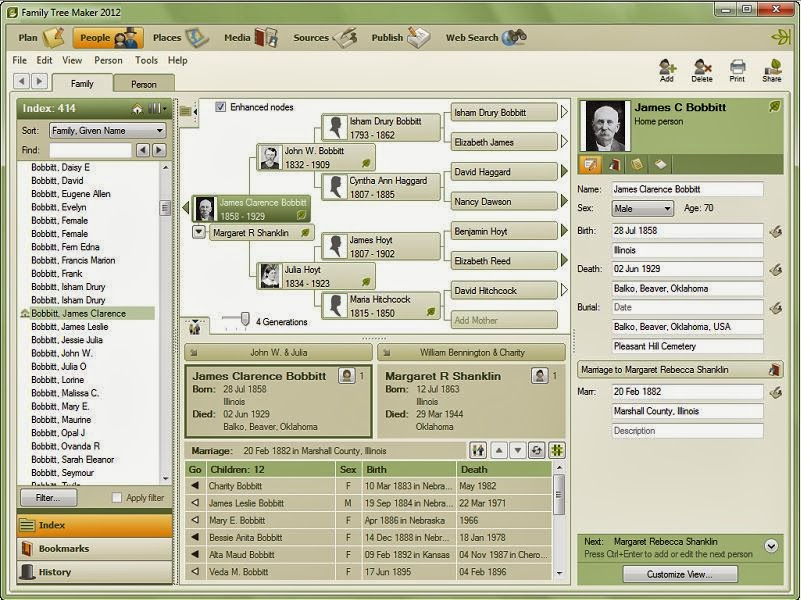
\includegraphics[width=\linewidth]{figs/ftmShot.png}
    \caption{Main Screen of Family Tree Maker}
    \label{fig:ftmShot}
\end{figure}

\begin{figure}
    \centering
    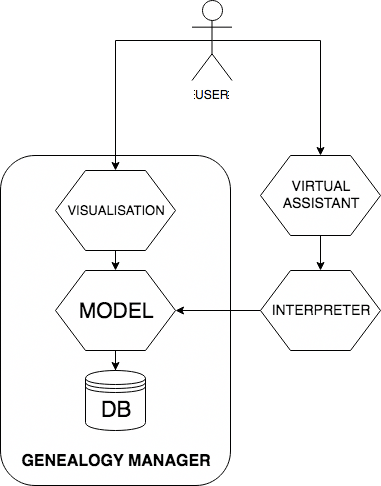
\includegraphics[width=\linewidth]{figs/structure.png}
    \caption{Structure of System Components}
    \label{fig:struct}
\end{figure}

\chapter{Documentation of Standard KISP Functions}
\label{chap:doc}
Note that two commas after a parameter name is a signature means any positive number of arguments. Also, a backtick (\texttt{`})
denotes a single quote (').

\subsection{void}
\begin{itemize}
    \item Name: Void Constant
    \item Signature: \texttt{void}
    \item Description: A unique constant of type Void.
    \item Examples :
        \begin{itemize}
            \item \texttt{(= void void) = true}
            \item \texttt{(= void 3) = false}
        \end{itemize}
    \item Type : \[Void\]
\end{itemize}

\subsection{define}
\begin{itemize}
    \item Name: Define
    \item Signature: \texttt{(define reference term)}
    \item Description: Creates an abbreviation \texttt{reference} for the specified lisp \texttt{term}.
    \item Arguments:
        \begin{itemize}
            \item \textbf{reference} : A shortcut for \texttt{term}. Can only be composed of lowercase English letters and a dash.
            \item \textbf{term} : A well-formed lisp term as a designatum. Keep in mind that you can use \texttt{reference} in \texttt{term} to create recursion, but make sure that there are no cyclic definitions.
        \end{itemize}
    \item Examples :
        \begin{itemize}
            \item \texttt{(define name 'John Doe')}
            \item \texttt{(define two 2)}
            \item \texttt{(define twice (lambda (n) (f (f n))))}
        \end{itemize}
    \item Type : \[Void\]
    \item Notes : This function cannot be used inside another functions, only as a top-level term. You cannot redefine standard keywords like define itself, \texttt{lambda} and so on.
\end{itemize}

\subsection{lambda}
\begin{itemize}
    \item Name: Lambda
    \item Signature: \texttt{(lambda (args) lambda-term)}
    \item Description: Instantiates a new anonymous function which takes its arguments \texttt{args} and applies them to the \texttt{term}
    \item Arguments:
        \begin{itemize}
            \item \textbf{args} : A list of argument names for this lambda-term separated by space
            \item \textbf{term} : A well-formed lisp term that will be applied to arguments \texttt{args}
        \end{itemize}
    \item Examples :
        \begin{itemize}
            \item \texttt{(lambda () 2)}
            \item \texttt{(lambda (n) (* 2 n)}
            \item \texttt{(lambda (a, b) (+ a (* a b))}
        \end{itemize}
    \item Notes : You can use only English letters and dashes for names of the arguments. Argument list is separated by single space. Empty argument list is permitted
\end{itemize}

\subsection{and}
\begin{itemize}
    \item Name: And
    \item Signature: \texttt{(and boolean..)}
    \item Description: Performs a logical AND operation on N boolean terms
    \item Arguments:
        \begin{itemize}
            \item \textbf{boolean1} : First boolean conjunct
            \item \textbf{boolean2} : Second boolean conjunct
            \item \textbf{...} : ...
            \item \textbf{booleanN} : N-th boolean conjunct
        \end{itemize}
    \item Examples :
        \begin{itemize}
            \item \texttt{(and true) = true}
            \item \texttt{(and false true) = false}
            \item \texttt{(and true true false) = false}
        \end{itemize}
    \item Type : \[(Boolean)^n  o Boolean\]
    \item Notes : All conjuncts will be evaluated, always. Function accepts any non-zero number of arguments.
\end{itemize}

\subsection{or}
\begin{itemize}
    \item Name: Or
    \item Signature: \texttt{Performs a logical OR operation on N boolean terms.}
    \item Description: (or boolean..)
    \item Arguments:
        \begin{itemize}
            \item \textbf{boolean1} : First boolean disjunct
            \item \textbf{boolean2} : Second boolean disjunct
            \item \textbf{booleanN} : N-th boolean disjunct
        \end{itemize}
    \item Examples :
        \begin{itemize}
            \item \texttt{(or true) = true}
            \item \texttt{(or false true) = true}
            \item \texttt{(or false false true) = true}
        \end{itemize}
    \item Type : \[(Boolean)^n \to Boolean\]
    \item Notes : All disjuncts will be evaluated, always. Function accepts any non-zero number of arguments.
\end{itemize}

\subsection{not}
\begin{itemize}
    \item Name: Not
    \item Signature: \texttt{(not boolean-term)}
    \item Description: Performs a logical NOT operation on exactly one boolean term.
    \item Arguments:
        \begin{itemize}
            \item \textbf{boolean} : A boolean term, whose value will be inverted.
        \end{itemize}
    \item Examples :
        \begin{itemize}
            \item \texttt{(not true) = false}
            \item \texttt{(not false) = true}
        \end{itemize}
    \item Type : \[Boolean \to Boolean\]
    \item Notes : This function accepts only one boolean argument.
\end{itemize}

\subsection{during}
\begin{itemize}
    \item Name: During
    \item Signature: \texttt{(during date-point date-star date-end)}
    \item Description: Checks whether the date \texttt{date-point} is after \texttt{date-start} and before \texttt{date-finish}. Returns \texttt{true} iff \texttt{date-point} belongs to the time interval [\texttt{date-start}, \texttt{date-date-end}]
    \item Arguments:
        \begin{itemize}
            \item \textbf{date-point} : A date which is going to be checked for belonging to the time interval [\texttt{date-start}, \texttt{date-end}]
            \item \textbf{date-start} : A starting point of the time interval
            \item \textbf{date-end} : An ending point of the time interval
        \end{itemize}
    \item Examples :
        \begin{itemize}
            \item \texttt{(during WWII 1900 2000) = true}
        \end{itemize}
    \item Type : \[(Date)^3 \to Boolean\]
    \item Notes :
\end{itemize}

\subsection{before}
\begin{itemize}
    \item Name: Before
    \item Signature: \texttt{(before date-pointA date-pointB)}
    \item Description: Checks whether date point A is happened before date point B. Returns true or false accordingly.
    \item Arguments:
        \begin{itemize}
            \item \textbf{date-pointA} : First time point, which is needed to be before the second point for the formula to result in \texttt{true}.
            \item \textbf{date-pointB} : Second time point
        \end{itemize}
    \item Examples :
        \begin{itemize}
            \item \texttt{(before WWII WWI) = false}
        \end{itemize}
    \item Type : \[(Date)^2 \to Boolean\]
    \item Notes :
\end{itemize}

\subsection{after}
\begin{itemize}
    \item Name: After
    \item Signature: \texttt{(after date-pointA date-pointB)}
    \item Description: Checks whether date point A is happened after date point B. Returns true or false accordingly.
    \item Arguments:
        \begin{itemize}
            \item \textbf{date-pointA} : First time point, which is needed to be after the second point for the formula to result in \texttt{true}.
            \item \textbf{date-pointB} : Second time point
        \end{itemize}
    \item Examples :
        \begin{itemize}
            \item \texttt{(after WWII WWI) = false}
        \end{itemize}
    \item Type : \[(Date)^2 \to Boolean\]
    \item Notes :
\end{itemize}

\subsection{date}
\begin{itemize}
    \item Name: Date
    \item Signature: \texttt{(date string-date)}
    \item Description: Parses \texttt{string-date} and returns a date object created from this string
    \item Arguments:
        \begin{itemize}
            \item \textbf{string-date} : A string representation of a date object. Should be in the format: dd.mm.year.
        \end{itemize}
    \item Examples :
        \begin{itemize}
            \item \texttt{(date '10.11.1995')}
            \item \texttt{(date '01.01.1900')}
        \end{itemize}
    \item Type : \[String \to Date\]
    \item Notes : You should strictly follow the date format in order for this function to work. Void is returned iff invalid string is passed to this function.
\end{itemize}

\subsection{list}
\begin{itemize}
    \item Name: List
    \item Signature: \texttt{(list args..)}
    \item Description: Creates a list object from passed arguments.
    \item Arguments:
        \begin{itemize}
            \item \textbf{args} : A space-separated list of objects out of which list will be created
        \end{itemize}
    \item Examples :
        \begin{itemize}
            \item \texttt{(list 1 2 3 4)}
            \item \texttt{(list 'first' 'second' 'third')}
            \item \texttt{(list 1 'two' (date '1.1.1990'))}
        \end{itemize}
    \item Type : \[(Object)^n \to List\]
    \item Notes : Accepts non-zero number of arguments. Parameters are allowed to be of different type. If you want an empty list, use the term \texttt{vacant}.
\end{itemize}

\subsection{join}
\begin{itemize}
    \item Name: Join
    \item Signature: \texttt{(join list..)}
    \item Description: Concatenates N lists
    \item Arguments:
        \begin{itemize}
            \item \textbf{list} : A space-separated sequence of lists to be concatenated
        \end{itemize}
    \item Examples :
        \begin{itemize}
            \item \texttt{(join list1 list2)}
            \item \texttt{(join list)}
            \item \texttt{(join (list 1 2) (list 3) (list 4)) = [1, 2, 3, 4]}
        \end{itemize}
    \item Type : \[(List)^n \to List\]
    \item Notes : Accepts non-zero number of arguments.
\end{itemize}

\subsection{count}
\begin{itemize}
    \item Name: Count
    \item Signature: \texttt{(count list)}
    \item Description: Returns the number of elements in \texttt{list}.
    \item Arguments:
        \begin{itemize}
            \item \textbf{list} : A list object.
        \end{itemize}
    \item Examples :
        \begin{itemize}
            \item \texttt{(count (list 1 2 3)) = 3}
            \item \texttt{(count (list 1)) = 1}
        \end{itemize}
    \item Type : \[List \to Numeral\]
    \item Notes : Accepts a non-zero number of arguments.
\end{itemize}

\subsection{filter}
\begin{itemize}
    \item Name: Filter
    \item Signature: \texttt{(filter predicate list)}
    \item Description: Takes a predicate together with a list and retains only those elements, which satisfy predicates' condition.
    \item Arguments:
        \begin{itemize}
            \item \textbf{predicate} : Lambda function of type $Object \to Boolean$, which we apply to all elements in \texttt{list}
            \item \textbf{list} : A list which needs to be filtered
        \end{itemize}
    \item Examples :
        \begin{itemize}
            \item \texttt{(filter odd? (list 1 2 3 4 5)) = [1, 3, 5]}
            \item \texttt{(filter uppercase? (list 'TEST' 'test' 'tEsT')) = ['TEST']}
        \end{itemize}
    \item Type : \[(Lambda \times List) \to List\]
\end{itemize}

\subsection{at}
\begin{itemize}
    \item Name: At
    \item Signature: \texttt{(at list index)}
    \item Description: Returns the \texttt{index}-th element of \texttt{list}.
    \item Arguments:
        \begin{itemize}
            \item \textbf{list index} : A list whose element at specified place will be taken
        \end{itemize}
    \item Examples :
        \begin{itemize}
            \item \texttt{(at (list 1 2 3 4) 3) = 4}
            \item \texttt{(at (list 0 1 2) 3) = void}
            \item \texttt{(at (list 0 1 2 3 4 5) -1) = 5}
        \end{itemize}
    \item Type : \[(List \times Numeral) \to Object\]
    \item Notes : Indices start with 0. If there is no item at specified index, then Void is returned. Indices can be negative, e.g. -1 points to last element, -2 -- penultimate, -3 -- antepenultimate and so on.
\end{itemize}

\subsection{append}
\begin{itemize}
    \item Name: Append
    \item Signature: \texttt{(append list item..)}
    \item Description: Includes all \texttt{item}s in the end of \texttt{list}.
    \item Arguments:
        \begin{itemize}
            \item \textbf{list} : A list to which items will be included
            \item \textbf{item..} : A space-separated sequence of objects that will be included in the \texttt{list}
        \end{itemize}
    \item Examples :
        \begin{itemize}
            \item \texttt{(append list 1)}
            \item \texttt{(append (list 1 2 3) 4 5 6) = [1, 2, 3, 4, 5, 6]}
        \end{itemize}
    \item Type : \[(List \times (Object)^n) \to List\]
    \item Notes : You can pass any positive number of arguments
\end{itemize}

\subsection{mod}
\begin{itemize}
    \item Name: Modulo
    \item Signature: \texttt{(mod a n)}
    \item Description: Computes a residue modulo \texttt{n}, i.e. the remainder of a natural division of \texttt{a} by \texttt{n}
    \item Arguments:
        \begin{itemize}
            \item \textbf{a} : Dividend
            \item \textbf{n} : Divisor
        \end{itemize}
    \item Examples :
        \begin{itemize}
            \item \texttt{(mod 5 2) = 1}
            \item \texttt{(mod 10 4) = 2}
        \end{itemize}
    \item Type : \[(Numeral)^2 \to Numeral\]
    \item Notes : Divisor should not be zero.
\end{itemize}

\subsection{add}
\begin{itemize}
    \item Name: Addition, or $+$
    \item Signature: \texttt{(+ number..)}
    \item Description: Calculates sum of all \texttt{number}s.
    \item Arguments:
        \begin{itemize}
            \item \textbf{number..} : A non-empty space-separated sequence of numeral terms.
        \end{itemize}
    \item Examples :
        \begin{itemize}
            \item \texttt{(+ 2) = 2}
            \item \texttt{(+ 1357 10) = 1367}
            \item \texttt{(+ 1 2 3) = 6}
        \end{itemize}
    \item Type : \[(Numeral)^n \to Numeral\]
    \item Notes : The function accepts any positive number of arguments
\end{itemize}

\subsection{mul}
\begin{itemize}
    \item Name: Multiplication, or $*$
    \item Signature: \texttt{(* number..)}
    \item Description: Calculates product of all \texttt{number}s.
    \item Arguments:
        \begin{itemize}
            \item \textbf{number..} : A non-empty space-separated sequence of numeral terms.
        \end{itemize}
    \item Examples :
        \begin{itemize}
            \item \texttt{(* 2) = 2}
            \item \texttt{(* 1357 10) = 13570}
            \item \texttt{(* 1 2 3) = 6}
        \end{itemize}
    \item Type : \[(Numeral)^n \to Numeral\]
    \item Notes : The function accepts any positive number of arguments
\end{itemize}

\subsection{lessEqual}
\begin{itemize}
    \item Name: Less Or Equal, $<=$
    \item Signature: \texttt{(<= a b)}
    \item Description: Checks whether \texttt{a} <= \texttt{b}
    \item Arguments:
        \begin{itemize}
            \item \textbf{a} : first numeral to be compared
            \item \textbf{b} : second numeral to be compared
        \end{itemize}
    \item Examples :
        \begin{itemize}
            \item \texttt{(<= 2 5) = true}
            \item \texttt{(<= 10 3) = false}
        \end{itemize}
    \item Type : \[(Numeral)^2 \to Boolean\]
    \item Notes : Function expects exactly two numerals as arguments.
\end{itemize}

\subsection{less}
\begin{itemize}
    \item Name: Less, or just $<$
    \item Signature: \texttt{(< a b)}
    \item Description: Checks whether $a < b$
    \item Arguments:
        \begin{itemize}
            \item \textbf{a} : first numeral to be compared
            \item \textbf{b} : second numeral to be compared
        \end{itemize}
    \item Examples :
        \begin{itemize}
            \item \texttt{(< 2 5) = true}
            \item \texttt{(< 10 3) = false}
        \end{itemize}
    \item Type : \[(Numeral)^2 \to Boolean\]
    \item Notes : Function expects exactly two numerals as arguments.
\end{itemize}

\subsection{greater}
\begin{itemize}
    \item Name: Greater, or just $>$
    \item Signature: \texttt{(> a b)}
    \item Description: Checks whether $a > b$
    \item Arguments:
        \begin{itemize}
            \item \textbf{a} : first numeral to be compared
            \item \textbf{b} : second numeral to be compared
        \end{itemize}
    \item Examples :
        \begin{itemize}
            \item \texttt{(> 5 2) = true}
            \item \texttt{(> 10 13) = false}
        \end{itemize}
    \item Type : \[(Numeral)^2 \to Boolean\]
    \item Notes : Function expects exactly two numerals as arguments.
\end{itemize}

\subsection{greaterOrEqual}
\begin{itemize}
    \item Name: Greater Or Equal, $>=$
    \item Signature: \texttt{(>= a b)}
    \item Description: Checks whether $a \ge b$
    \item Arguments:
        \begin{itemize}
            \item \textbf{a} : first numeral to be compared
            \item \textbf{b} : second numeral to be compared
        \end{itemize}
    \item Examples :
        \begin{itemize}
            \item \texttt{(>= 5 5) = true}
            \item \texttt{(>= 3 5) = false}
        \end{itemize}
    \item Type : \[(Numeral)^2 \to Boolean\]
    \item Notes : Function expects exactly two numerals as arguments.
\end{itemize}

\subsection{concat}
\begin{itemize}
    \item Name: String Concatenation
    \item Signature: \texttt{(concat string..)}
    \item Description: Concatenates all \texttt{string}s
    \item Arguments:
        \begin{itemize}
            \item \textbf{string} : A non-empty space-separated sequence of string objects.
        \end{itemize}
    \item Examples :
        \begin{itemize}
            \item \texttt{(concat 'test' 'ing' ' concat') = 'testing concat'}
            \item \texttt{(concat 'hello ' 'world!') = 'hello world!'}
        \end{itemize}
    \item Type : \[(String)^n \to String\]
    \item Notes : This function accepts any positive number of arguments.
\end{itemize}

\subsection{of-type?}
\begin{itemize}
    \item Name: Of Type?
    \item Signature: \texttt{(of-type? o type)}
    \item Description: Returns true iff object \texttt{o} has a \texttt{type}.
    \item Arguments:
        \begin{itemize}
            \item \textbf{o type} : An object whose type needs to be checked
            \item \textbf{type} : A name of a type
        \end{itemize}
    \item Examples :
        \begin{itemize}
            \item \texttt{(of-type? 'test' 'string) = true}
            \item \texttt{(of-type? 3 'date') = false}
        \end{itemize}
    \item Type : \[(Object \times String) \to Boolean\]
    \item Notes : The name of a type should be entered precisely
\end{itemize}

\subsection{equals}
\begin{itemize}
    \item Name: Equals, or $=$
    \item Signature: \texttt{(= objA objB)}
    \item Description: Returns true iff \texttt{objA} and \texttt{objB} are exactly the same thing.
    \item Arguments:
        \begin{itemize}
            \item \textbf{objA} : First object to be compared
            \item \textbf{objB} : Second object to be compared
        \end{itemize}
    \item Examples :
        \begin{itemize}
            \item \texttt{(= '3' 3) = false}
            \item \texttt{(= 10 10) = true}
            \item \texttt{(= (date '1.1.1999') (date '1.1.1999')) = true}
        \end{itemize}
    \item Type : \[(Object)^2 \to Boolean\]
    \item Notes : Function accepts exactly two arguments
\end{itemize}

\subsection{sub}
\begin{itemize}
    \item Name: Subtraction, or $-$
    \item Signature: \texttt{(sub m s)}
    \item Description: Calculates the difference between m (minuend) and s (subtrahend).
    \item Arguments:
        \begin{itemize}
            \item \textbf{m} : Minuend
            \item \textbf{s} : Subtrahend
        \end{itemize}
    \item Examples :
        \begin{itemize}
            \item \texttt{(sub 5 2) = 3}
            \item \texttt{(sub 0 1) = -1}
        \end{itemize}
    \item Type : \[(Numeral)^2 \to Numeral\]
    \item Notes : Accepts exactly two arguments.
\end{itemize}

\subsection{div}
\begin{itemize}
    \item Name: Integer division
    \item Signature: \texttt{(div n m)}
    \item Description: Calculates the quotient from integer division of n (dividend) by m (divisor)
    \item Arguments:
        \begin{itemize}
            \item \textbf{n} : Dividend
            \item \textbf{m} : Divisor
        \end{itemize}
    \item Examples :
        \begin{itemize}
            \item \texttt{(div 10 2) = 5}
            \item \texttt{(div 5 2) = 2}
            \item \texttt{(div 3 2) = 1}
        \end{itemize}
    \item Type : \[(Numeral)^2 \to Numeral\]
    \item Notes : Accepts exactly two arguments. Divisor shouldn't be zero, or exception will be thrown
\end{itemize}

\subsection{father}
\begin{itemize}
    \item Name: Father
    \item Signature: \texttt{(father person)}
    \item Description: Returns father of the specified person
    \item Arguments:
        \begin{itemize}
            \item \textbf{person} : A link to a person object
        \end{itemize}
    \item Examples :
        \begin{itemize}
            \item \texttt{(father (person 'John' 'Golt'))}
            \item \texttt{(father (person 'Emma Clark'))}
        \end{itemize}
    \item Type : \[Person \to Person\]
    \item Notes : Accepts and returns exactly one object of type Person. If provided person doesn't have a father, returns empty
        list.
\end{itemize}

\subsection{mother}
\begin{itemize}
    \item Name: Mother
    \item Signature: \texttt{(mother person)}
    \item Description: Returns mother of the specified person
    \item Arguments:
        \begin{itemize}
            \item \textbf{person} : A link to a person object
        \end{itemize}
    \item Examples :
        \begin{itemize}
            \item \texttt{(mother (person 'John' 'Golt'))}
            \item \texttt{(mother (person 'Emma Clark'))}
        \end{itemize}
    \item Type : \[Person \to Person\]
    \item Notes : Accepts and returns exactly one object of type Person. If provided person doesn't have a mother, returns empty
        list.
\end{itemize}

\subsection{spouse}
\begin{itemize}
    \item Name: Spouse
    \item Signature: \texttt{(spouse person)}
    \item Description: Returns spouse of the specified person
    \item Arguments:
        \begin{itemize}
            \item \textbf{person} : A link to a person object
        \end{itemize}
    \item Examples :
        \begin{itemize}
            \item \texttt{(spouse (person 'John' 'Golt'))}
            \item \texttt{(spouse (person 'Emma Clark'))}
        \end{itemize}
    \item Type : \[Person \to Person\]
    \item Notes : Accepts and returns exactly one object of type Person. If provided person doesn't have a spouse, returns empty
        list.
\end{itemize}

\subsection{children}
\begin{itemize}
    \item Name: Children
    \item Signature: \texttt{(children person)}
    \item Description: Returns list of persons' children
    \item Arguments:
        \begin{itemize}
            \item \textbf{person} : A link to a person object
        \end{itemize}
    \item Examples :
        \begin{itemize}
            \item \texttt{(children (person 'John' 'Golt'))}
            \item \texttt{(children (person 'Emma Clark'))}
        \end{itemize}
    \item Type : \[Person \to List\]
    \item Notes : Returns empty list if the specified person is childless.
\end{itemize}

\subsection{gen-dist}
\begin{itemize}
    \item Name: Generation Distance
    \item Signature: \texttt{(gen-dist person1 person2)}
    \item Description: Calculates the \texttt{generation distance} between two people
    \item Arguments:
        \begin{itemize}
            \item \textbf{person1} : First person
            \item \textbf{person2} : Second person
        \end{itemize}
    \item Examples :
        \begin{itemize}
            \item \texttt{(gen-dist me (father me)) = -1}
            \item \texttt{(gen-dist me (grandfather me)) = -2}
            \item \texttt{(gen-dist me (son me)) = 1}
        \end{itemize}
    \item Type : \[(Person)^2 \to Numeral\]
    \item Notes : Generation distance is the difference between generations. The generation of the first person is assumed to be zero, and the generation of the second person is calculated accordingly.
\end{itemize}

\subsection{person}
\begin{itemize}
    \item Name: Person
    \item Signature: \texttt{(person first-name)}
    \item Description: Returns the person with specified first and last name
    \item Arguments:
        \begin{itemize}
            \item \textbf{first-name} : A string with the first name of a person
        \end{itemize}
    \item Examples :
        \begin{itemize}
            \item \texttt{(person 'John' 'Doe')}
        \end{itemize}
    \item Type : \[String^2 \to Person\]
    \item Notes : The function also accepts full name in one string: (person 'Full Name')
\end{itemize}

\subsection{kinship}
\begin{itemize}
    \item Name: Kinship
    \item Signature: \texttt{(kinship person1 person2)}
    \item Description: Returns a list of basic kinship terms (strings) that represents how is \texttt{person1} related to \texttt{person2}.
    \item Arguments:
        \begin{itemize}
            \item \textbf{person1 person2} : First person
        \end{itemize}
    \item Examples :
        \begin{itemize}
            \item \texttt{(kinship (father me) me) = ['father']}
            \item \texttt{(kinship (uncle me) me) = ['son','parent','parent']}
        \end{itemize}
    \item Type : \[Person^2 \to List\]
    \item Notes : Basic kinship terms are: \texttt{father}, \texttt{mother}, \texttt{parent}, \texttt{son}, \texttt{daughter}, \texttt{child}, \texttt{husband}, \texttt{wife}, \texttt{spouse}
\end{itemize}

\subsection{attr}
\label{doc:attr}
\begin{itemize}
    \item Name: Get Attribute
    \item Signature: \texttt{(attr person prop)}
    \item Description: Returns requested property \texttt{prop} of the specified \texttt{person}.
    \item Arguments:
        \begin{itemize}
            \item \textbf{person} : Person of interest
            \item \textbf{prop} : Property of interest
        \end{itemize}
    \item Examples :
        \begin{itemize}
            \item \texttt{(attr (person 'John Golt') 'first name') = 'John'}
            \item \texttt{(attr (person 'John Golt') 'sex') = 'MALE'))}
        \end{itemize}
    \item Type : \[(Person \times String) \to Object\]
    \item Notes : All possible properties are: \texttt{first name}, \texttt{last name}, \texttt{full name}, \texttt{second name},
        \texttt{birth}, \texttt{birth date}, \texttt{date of birth}, \texttt{gender}, \texttt{sex}, \texttt{birthplace}, \texttt{phone}, \texttt{phone number}, \texttt{tel}, \texttt{email}, \texttt{e-mail}, \texttt{wedding}.
\end{itemize}

\subsection{shorten}
\begin{itemize}
    \item Name: Shorten Kinship Term
    \item Signature: \texttt{(shorten list)}
    \item Description: Reduces the list of basic kinship terms.
    \item Arguments:
        \begin{itemize}
            \item \textbf{list} : List of basic kinship terms.
        \end{itemize}
    \item Examples :
        \begin{itemize}
            \item \texttt{(shorten (kinship person1 person2))}
        \end{itemize}
    \item Type : \[List \to List\]
    \item Notes :
\end{itemize}

\subsection{put-kinship-term}
\begin{itemize}
    \item Name: Put Kinship Term
    \item Signature: \texttt{(put-kinship-term list-basic shortcut)}
    \item Description: Registers a new custom kinship term \texttt{shortcut} from the list of basic terms \texttt{list-basic}. The new term can be used later in \texttt{shorten} function.
    \item Arguments:
        \begin{itemize}
            \item \textbf{list-basic} : Non-empty list of basic kinship terms
            \item \textbf{shortcut} : A string with a definition of a new kinship term
        \end{itemize}
    \item Examples :
        \begin{itemize}
            \item \texttt{(put-kinship-term (list 'son' 'parent' 'parent') 'uncle')}
            \item \texttt{(put-kinship-term (list 'son' 'parent') 'brother')}
        \end{itemize}
    \item Type : \[Void\]
    \item Notes :
\end{itemize}

\subsection{vacant}
\begin{itemize}
    \item Name: Vacant List
    \item Description: An empty list constant
    \item Examples :
        \begin{itemize}
            \item \texttt{(count vacant) = 0}
        \end{itemize}
    \item Type : \[List\]
\end{itemize}

\subsection{map}
\begin{itemize}
    \item Name: List Mapping Function
    \item Signature: \texttt{(map f list) or (map f l1 l2)}
    \item Description: Applies the unary function f to each element of a specified list or constructs a third list by applying binary f to each consecutive pair of elements from lists l1 and l2.
    \item Arguments:
        \begin{itemize}
            \item \textbf{f} : An unary or binary mapping function
            \item \textbf{list} : A list whose elements will be mapped one by one
            \item \textbf{l1} : A list, each item of which will be supplied to f as a first argument
            \item \textbf{l2} : A list, each item of which will be supplied to f as a second argument
        \end{itemize}
    \item Examples :
        \begin{itemize}
            \item \texttt{(map square (first-n 3)) = [1, 4, 9]}
            \item \texttt{(map + (list 1 2 3) (list 4 5 6)) = [5, 7, 9]}
        \end{itemize}
    \item Type : \[Either Lambda \times List \to List or Lambda \times (List)^2 \to List\]
    \item Notes :
\end{itemize}

\subsection{tail}
\begin{itemize}
    \item Name: Tail
    \item Signature: \texttt{(tail list)}
    \item Description: Return the tail, i.e. all but the first element of a list
    \item Arguments:
        \begin{itemize}
            \item \textbf{list} : A specified list
        \end{itemize}
    \item Examples :
        \begin{itemize}
            \item \texttt{(tail (list 0 1 2)) = (list 1 2)}
            \item \texttt{(tail (list 1)) = vacant}
        \end{itemize}
    \item Type : \[List \to List\]
    \item Notes : This function is analogous to \texttt{cdr} in Common Lisp.
\end{itemize}

\subsection{head}
\begin{itemize}
    \item Name: Head
    \item Signature: \texttt{(head list)}
    \item Description: Returns the head, i.e. the first element of a list
    \item Arguments:
        \begin{itemize}
            \item \textbf{list} : A specified list
        \end{itemize}
    \item Examples :
        \begin{itemize}
            \item \texttt{(head (list 1 2 3))= 1}
            \item \texttt{(head vacant) = void}
        \end{itemize}
    \item Type : \[List \to Object\]
    \item Notes : This function is analogous to \texttt{car} in Common Lisp.
\end{itemize}

\subsection{now}
\begin{itemize}
    \item Name: Now
    \item Signature: \texttt{now}
    \item Description: A date constant that hold the current time.
    \item Examples :
        \begin{itemize}
            \item \texttt{(before now now) = false}
        \end{itemize}
    \item Type : \[Date\]
\end{itemize}

\subsection{people}
\begin{itemize}
    \item Name: People
    \item Signature: \texttt{people}
    \item Description: A constant of type List that holds all persons in a family tree.
    \item Examples :
        \begin{itemize}
            \item \texttt{(head people)}
        \end{itemize}
    \item Type : \[List\]
\end{itemize}

\subsection{string}
\begin{itemize}
    \item Name: String
    \item Signature: \texttt{(string numeral)}
    \item Description: Converts given integer to string.
    \item Arguments:
        \begin{itemize}
            \item \textbf{numeral} : A specified integer.
        \end{itemize}
    \item Examples :
        \begin{itemize}
            \item \texttt{(string 12) = '12'}
            \item \texttt{(string 10000) = '10000'}
        \end{itemize}
    \item Type : \[Numeral \to String\]
\end{itemize}

\subsection{substr}
\begin{itemize}
    \item Name: Sub-string
    \item Signature: \texttt{(substr source start [end])}
    \item Description: Return a substring of the specified source, starting from `start` and ending just before `end`.
    \item Arguments:
        \begin{itemize}
            \item \textbf{source} : A super-string, from which we want to get a sub-string
            \item \textbf{start} : An inclusive starting index of the substring. Should be positive.
            \item \textbf{end} : An optional exclusive ending index of the substring. Should be positive and not less than
                `start`.
        \end{itemize}
    \item Examples :
        \begin{itemize}
            \item \texttt{(substr '01234' 0 0) = ''}
            \item \texttt{(substr '01234' 0 2) = '01'}
            \item \texttt{(substr '01234' 1 3) = '13'}
            \item \texttt{(substr '01234' 1) = '1234'}
        \end{itemize}
    \item Type : \[String \times Numeral \times Numeral \to String\]
    \item Note : The last argument can be omitted, resulting in it being equal to the length of a source string.
\end{itemize}

\subsection{day}
\begin{itemize}
    \item Name: Day of month
    \item Signature: \texttt{(day date)}
    \item Description: Return the day of a month of the specified date as a numeral.
    \item Arguments:
        \begin{itemize}
            \item \textbf{date} : A date object, whose day component is needed.
        \end{itemize}
    \item Examples :
        \begin{itemize}
            \item \texttt{(day (date '1.2.2000')) = 1}
            \item \texttt{(day (date '25.3.2001')) = 25}
        \end{itemize}
    \item Type : \[ Date \to Numeral \]
\end{itemize}

\subsection{month}
\begin{itemize}
    \item Name: Month
    \item Signature: \texttt{(month date)}
    \item Description: Return the month of the specified date as a numeral.
    \item Arguments:
        \begin{itemize}
            \item \textbf{date} : A date object, whose month component is needed.
        \end{itemize}
    \item Examples :
        \begin{itemize}
            \item \texttt{(month (date '1.2.2000')) = 2}
            \item \texttt{(month (date '25.3.2001')) = 3}
        \end{itemize}
    \item Type : \[ Date \to Numeral \]
\end{itemize}

\subsection{year}
\begin{itemize}
    \item Name: Year
    \item Signature: \texttt{(year date)}
    \item Description: Return the year of the specified date as a numeral.
    \item Arguments:
        \begin{itemize}
            \item \textbf{year} : A date object, whose year component is needed.
        \end{itemize}
    \item Examples :
        \begin{itemize}
            \item \texttt{(year (date '1.2.2000')) = 2000}
            \item \texttt{(year (date '25.3.2001')) = 2001}
        \end{itemize}
    \item Type : \[ Date \to Numeral \]
\end{itemize}
